\documentclass[tikz,border=10pt]{standalone}

\newcommand{\comment}[1]{}

\usepackage{tikz}
\usetikzlibrary{positioning, calc,shadows,patterns,snakes}

\makeatletter
\pgfdeclareshape{document}{
\inheritsavedanchors[from=rectangle] % this is nearly a rectangle
\inheritanchorborder[from=rectangle]
\inheritanchor[from=rectangle]{center}
\inheritanchor[from=rectangle]{north}
\inheritanchor[from=rectangle]{south}
\inheritanchor[from=rectangle]{west}
\inheritanchor[from=rectangle]{east}
\inheritanchor[from=rectangle]{south east}
\inheritanchor[from=rectangle]{south west}
% ... and possibly more
\backgroundpath{% this is new
% store lower right in xa/ya and upper right in xb/yb
\southwest \pgf@xa=\pgf@x \pgf@ya=\pgf@y
\northeast \pgf@xb=\pgf@x \pgf@yb=\pgf@y
% compute corner of ‘‘flipped page’’
\pgf@xc=\pgf@xb \advance\pgf@xc by-3.5pt % this should be a parameter
\pgf@yc=\pgf@yb \advance\pgf@yc by-3.5pt
% construct main path
\pgfpathmoveto{\pgfpoint{\pgf@xa}{\pgf@ya}}
\pgfpathlineto{\pgfpoint{\pgf@xa}{\pgf@yb}}
\pgfpathlineto{\pgfpoint{\pgf@xc}{\pgf@yb}}
\pgfpathlineto{\pgfpoint{\pgf@xb}{\pgf@yc}}
\pgfpathlineto{\pgfpoint{\pgf@xb}{\pgf@ya}}
\pgfpathclose
% add little corner
\pgfpathmoveto{\pgfpoint{\pgf@xc}{\pgf@yb}}
\pgfpathlineto{\pgfpoint{\pgf@xc}{\pgf@yc}}
\pgfpathlineto{\pgfpoint{\pgf@xb}{\pgf@yc}}
\pgfpathlineto{\pgfpoint{\pgf@xc}{\pgf@yc}}
}
}
\makeatother

\def\foldedpaper#1{
    \tikz[scale=#1,line width={#1*1pt}]{
        \def\a{1.41} % relative height
        \def\b{0.2}  % relative height/width of corner
        \def\c{0.1}  % relative margin width (on either side)
        \def\d{0.05} % vertical offset of lines
        \def\N{6}    % number of lines
        \draw         (0,0)
                --  ++(-1,0)
                --  ++(0,\a)
                --  ++(1-\b,0)
                --  ++(\b,-\b)
                -- cycle;
        \foreach \lnum in {1,...,\N}{
            \pgfmathsetmacro\yline{\a-\d-\lnum*\a/(\N+1)}
            \draw (-1+\c,\yline) -- (-\c,\yline);
        }
        \draw[fill=white] (0,\a-\b) -- ++(-\b,0) -- ++ (0,\b);
    }
}


\begin{document}
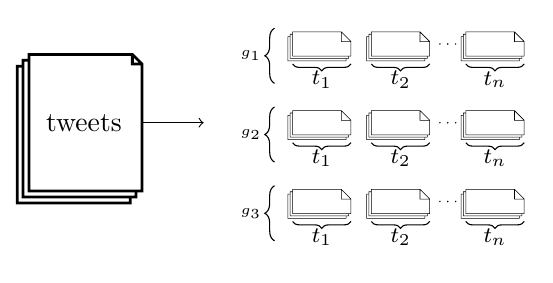
\begin{tikzpicture}
\tikzstyle{ground}=[fill,pattern=north east lines,draw=none,minimum width=0.3,minimum height=0.6]

\coordinate (posTweets) at (0,0);
\node (mytweets) [
  shape=document,
  double copy shadow={
    shadow xshift=-0.5ex,
    shadow yshift=-0.5ex
  },
  draw,
  fill=white,
  line width=1pt,
  text width=1cm,
  minimum height=1.7cm,
  minimum width=1.4cm
  ] at (posTweets) {tweets};

\coordinate (box2) at (2,2);

\foreach \j in {1,2,3}{

	\coordinate (posSeg) at ($(box2)-(0,\j)$);
	
	\draw [decorate,decoration={brace,amplitude=3.5pt}] 
	($(posSeg)+(0.4,-0.5)$) -- ($(posSeg)+(0.4,+0.2)$) node [black,midway,xshift=-0.3cm] {\tiny $g_{\j}$};
	
	\foreach \i in {1,2}{
	
		\node (anch) [
		  shape=document,
		  double copy shadow={
		    shadow xshift=-0.2ex,
		    shadow yshift=-0.2ex
		  },
		  draw,
		  fill=white,
		  line width=0.2pt,
		  text width=0.5cm,
		  minimum height=0.3cm
		  ] at ($ (posSeg)+(\i,0) $) {};

		\draw [decorate,decoration={brace,amplitude=2.5pt},xshift=0pt,yshift=-2pt] 
		($(anch.south east)+(0,-0.1)$) -- ($(anch.south west)+(0,-0.1)$) node [black,midway,yshift=-0.2cm] {\footnotesize $t_{\i}$};
	}

	\foreach \k in {2.5,2.6,2.7}{
		\node (d1) at ($(posSeg)+(\k,0)$) {};
		\fill (d1) circle [radius=0.3pt];	
	}

	\node (anch) [
	  shape=document,
	  double copy shadow={
	    shadow xshift=-0.2ex,
	    shadow yshift=-0.2ex
	  },
	  draw,
	  fill=white,
	  line width=0.2pt,
	  text width=0.5cm,
	  minimum height=0.3cm
	  ] at ($ (posSeg)+(3.2,0) $) {};

	\draw [decorate,decoration={brace,amplitude=2.5pt},xshift=0pt,yshift=-2pt] 
	($(anch.south east)+(0,-0.1)$) -- ($(anch.south west)+(0,-0.1)$) node [black,midway,yshift=-0.2cm] {\footnotesize $t_{n}$};
	
}

\draw [->] (mytweets.east) -- ($(box2)-(0.5,2)$);
\comment{
	\draw [
	    snake=coil,
	    segment amplitude=5pt,
	    segment length=5pt
	] (mytweets.south east) -- (10,0); 
	\draw [
	    thick,
	    decoration={
		brace,
		mirror,
		raise=0.5cm
	    },
	    decorate
	] (mytweets.north east) -- (10,0) 
	node [pos=0.5,anchor=north,yshift=-0.55cm] {coil}; 
}
\end{tikzpicture}
\end{document}
